\documentclass{exam}

\usepackage{amsmath,amssymb,amsfonts,amsthm,dsfont}
\usepackage{lib/extra}
\usepackage{graphicx}
\usepackage{tikz}
\usepackage{enumitem}
\usepackage{bbm}
\usepackage{pgfplots}

\pgfplotsset{compat=1.18}

\title{MTH 464 HW 5}
\author{Brandyn Tucknott}
\date{21 February 2025}

\begin{document}
\maketitle

\begin{questions}
    \question
Let $X, Y\sim$ Exp$(\lambda)$ be iid.

\begin{parts}
    \part Find the joint pdf of $U, V$.
    \sol
    First, compute the jacobian:
    $$J = \paren{\begin{matrix}
        \frac{\partial U}{\partial X} & \frac{\partial U}{\partial Y} \\
        \\
        \frac{\partial V}{\partial X} & \frac{\partial V}{\partial Y} \\
    \end{matrix}} = \paren{\begin{matrix}
        1 & 1 \\ -1 & 1 \\
    \end{matrix}} \longrightarrow \abs{\frac{1}{\det J}} = \frac{1}{2}$$

    Observe also that $x = \frac{u - v}{2}, y = \frac{u + v}{2}$. Then
    $$f_{U, V}(u, v) = f_{X, Y}\paren{x = \frac{u - v}{2}, y = \frac{u + v}{2}}\abs{\frac{1}{\det J}} = \lambda e^{-\lambda\frac{u - v}{2}}\lambda e^{-\lambda\frac{u + v}{2}}\cdot \frac{1}{2} = \frac{\lambda^2}{2} e^{-\lambda u}$$

    \part Show $U, V$ are uncorrelated but not independent.
    \sol
    To compute correlation, first compute the covariance.
    $$\cov{U}{V} = \cov{X + Y}{Y - X} = \cov{X}{Y} - \cov{X}{X} + \cov{Y}{Y} - \cov{Y}{X} = \var{Y} - \var{X} = 0$$
    Since $X, Y$ are iid. This allows us to conclude that $\corr{U}{V} = 0$.

    To find wether or not $U, V$ are independent, we will consider the region of $U, V$. Since it looks like

\begin{center}
    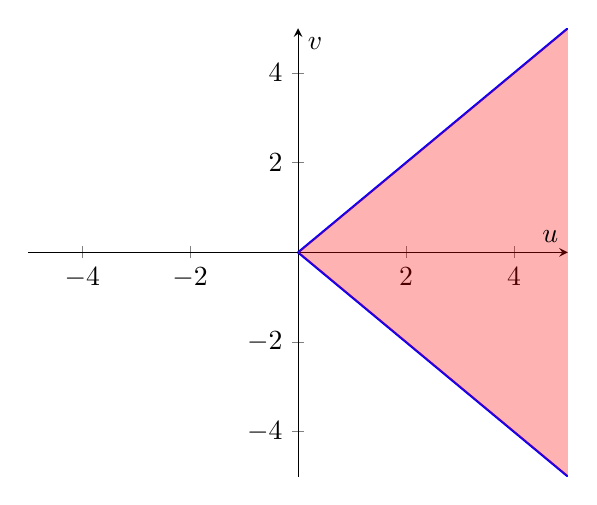
\begin{tikzpicture}
    \begin{axis}[
        axis lines=middle,
        xmin=-5, xmax=5,
        ymin=-5, ymax=5,
        samples=100,
        domain=0:5,
        xlabel={$u$},
        ylabel={$v$},
        legend pos=north east
    ]
    \addplot[blue, thick] {x};
    \addplot[blue, thick] {-x};
    \fill[red, opacity=0.3] (0, 0) -- (5, 5) -- (5, -5) -- (0, 0);
    \end{axis}
    \end{tikzpicture}
\end{center}
Since the region $U, V$ is not rectangular, and hence not a Cartesian product, we conclude $U, V$ are not independent.
\end{parts}
\newpage
\question
Let $\cbrac{U_j}_{j = 1}^\infty \sim \text{Unif}[0, 1]$ be iid. For $0 \leq x \leq 1$, define $N(x) = \min \cbrac{n : \sum_{k = 1}^n U_k > x}$. Note that by convention, $\sum_{k = 1}^0 U_k = 0, \text{ and also }P(N(x) \geq 1 = 1)$.

\begin{parts}
    \part Find $P(N(x) \geq 2)$.
    \sol
    Observe that
    $$P(N(x) \geq 2) = P\paren{\sum_{k = 1}^1 U_k \leq x} = P(U_1 \leq x) = x$$

    

    \part Show by induction that $P(N(x) \geq n + 1) = \frac{x^n}{n!}$.
    \begin{proof}
        We will first show by induction that $f_{\sum^n U_k}(x) = \frac{x^{n - 1}}{(n - 1)!}$ for $0 \leq x \leq n$ and $U_j\sim$ Unif[0, 1]. For a base case, it is obvious that if $k = 1$, then $f_{U_1} = \frac{x^0}{0!} = 1$, which mateches with the pdf for a std uniform distribution. Now assume the relation holds up to $n - 1$. We want to show it holds for $n$.
        \begin{align*}
            f_{\sum^n U_k} &= f_{\sum^{n - 1} U_k + U_n} \\
            &= \int_0^x f_{\sum^{n - 1}U_k}(x - u)f_{U_k}(u)du \\
            &= \int_0^x \frac{(x - u)^{n - 2}}{(n - 2)!}du \text{ let }v = x - u, dv = -du\\
            &= -\int_x^0 \frac{v^{n - 2}}{(n - 2)!}dv = \int_0^x \frac{v^{n - 2}}{(n - 2)!}dv \\
            &= \frac{x^{n - 1}}{(n - 1)!}
        \end{align*}

        Thus, we have shown that
        \begin{equation}
            f_{\sum^n U_k}(x) = \frac{x^{n - 1}}{(n - 1)!}\text{, for }0\leq x\leq n
        \end{equation}

        Now using equation (1) we directly compute
        \begin{align*}
            P\paren{N(x) \geq n + 1} &= P\paren{\sum_{k = 1}^n U_k \leq x} \\
            &= \int_0^x f_{\sum^n U_k}(x - u)f_U(u)du = \int_0^x f_{\sum^n U_k}(x - u)du = \int_0^x \frac{(x - u)^{n - 1}}{(n - 1)!}du\text{, let }v = x - u \\
            &= -\int_x^0 \frac{v^{n - 1}}{(n - 1)!}dv = \int_0^x \frac{v^{n - 1}}{(n - 1)!}dv = \frac{x^n}{n!}
        \end{align*}
    \end{proof}

    \part Recall that if $N$ is a positive integer valued random variable, then $E(N) = \sum_{k = 1}^\infty P(N(x) \geq k)$. Conclude that $E(N) = e^x$.
    \begin{proof}
        We directly calculate calculate $E(N)$ using our result from Part (b).
        \begin{align*}
            E(N) &= \sum_{k = 1}^\infty P(N(x) \geq k) \\
            &= \sum_{k = 1}^\infty \frac{x^{k - 1}}{(k - 1)!} \\
            &= \sum_{j = 0}^\infty \frac{x^j}{j!} = e^x
        \end{align*}
    \end{proof}
\end{parts}


\newpage
\question
Let $\cbrac{U_j}_{j = 1}^n\sim\text{Unif}[0, 1]$ be iid and $U_{(j)}, j = 1, 2, \hdots, n$ be its order values. Recall that the pdf of $U_{(j)}$ is given by
$$f_{U_{(j)}}(u) = \frac{n!}{(j - 1)!(n - j)!}u^{j - 1} (1 - u)^{n - j} \ind_{[0, 1]}(u)$$
Recall also that for all $a > 0, b > 0, \int_0^1 u^{a - 1}(1 - u)^{b - 1} du = \frac{\Gamma (a)\Gamma (b)}{\Gamma (a + b)}$

\begin{parts}
    \part Find $\E{U_{(j)}}$ and $\var{U_{(j)}}$.
    \sol
    \begin{align*}
        \E{U_{(j)}} &= \int_0^1 u\cdot \frac{n!}{(j - 1)!(n - j)!}u^{j - 1} (1 - u)^{n - j} du \\
        &= \frac{n!}{(j - 1)!(n - j)!} \int_0^1 u^j (1 - u)^{n - j} du \\
        &= \frac{n!}{(j - 1)!(n - j)!} \frac{\Gamma (j + 1) \Gamma (n - j + 1)}{\Gamma (n)} \\
        &= \frac{n!}{(j - 1)!(n - j)!}\frac{j!(n - j)!}{(n + 1)!} \\
        &= \frac{j}{n + 1}
    \end{align*}
    To compute the variance we need to quickly compute the $\E{U_{(j)}^2}$
    \begin{align*}
        \E{U_{(j)}^2} &= \int_0^1 u^2\cdot \frac{n!}{(j - 1)!(n - j)!}u^{j - 1} (1 - u)^{n - j} du \\
        &= \frac{n!}{(j - 1)!(n - j)!} \int_0^1 u^{j + 1} (1 - u)^{n - j} du \\
        &= \frac{n!}{(j - 1)!(n - j)!} \frac{\Gamma (j + 2) \Gamma (n - j + 1)}{\Gamma (n + 3)} \\
        &= \frac{n!}{(j - 1)!(n - j)!} \frac{(j + 1)!(n - j)!}{(n + 2)!} \\
        &= \frac{(j + 1)j}{(n + 2)(n + 1)}
    \end{align*}
    Finally, we compute the variance to be
    \begin{align*}
        \var{U_{(j)}} &= \E{U_{(j)}^2} - \paren{\E{U_{(j)}}}^2 \\
        &= \frac{j(j + 1)}{(n + 2)(n + 1)} - \paren{\frac{j}{n + 1}}^2 \\
        &= \frac{j(j + 1)}{(n + 2)(n + 1)} - \frac{j^2}{(n + 1)^2} \\
        &= \frac{j(j + 1)(n + 1) - j^2(n + 2)}{(n + 1)^2(n + 2)} \\
        &= \frac{j(n - j + 1)}{(n + 1)^2(n + 2)}
    \end{align*}

    \newpage % most of the old page is taken up
    \part Determine the value of $j$ that minimizes $\var{U_{(j)}}$.
    \sol
    Recognize first that the variance formula written in terms of $j$ can be expanded to
    \begin{align*}
        \var{U_{(j)}} &= \frac{j(n - j + 1)}{(n + 1)^2(n + 2)} \\
        &= \frac{-j^2 + jn + j}{(n + 1)^2(n + 2)}
    \end{align*}
    This is clearly a downward opening parabola, which means the minimum values will be at the endpoints, $j = 1, n$. They will be the same value because the variance is maximal at the vertex which can easily be shown to be equidistant from $j = 1, n$.
\end{parts}

\newpage
\question
Suppose that conditioned on $Y = y$, $X_1, X_2$ are independent random variables with mean $y$. Show that $\cov{X_1}{X_2} = \var{Y}$.
\begin{proof}
    We are given that conditioned on $Y = y$, then $X_1, X_2$ are independent with mean $y$. Note that this means $\E{X_1 | Y} = \E{X_2 | Y} = Y$.
    \begin{align*}
        \cov{X_1}{X_2} &= \E{X_1X_2} - \E{X_1}\E{X_2} \\
        &= \E{\E{X_1X_2 | Y}} - \E{\E{X_1 | Y}}\E{X_2 | Y} \\
        &= \E{\E{X_1 | Y}\E{X_2 | Y}} - \E{\E{X_1 | Y}}\E{\E{X_2 | Y}} \\
        &= \cov{\E{X_1 | Y}}{\E{X_2 | Y}} \\
        &= \cov{Y}{Y} = \var{Y}
    \end{align*}
\end{proof}



\newpage
\question
Show that $\cov{X}{\E{Y | X}} = \cov{X}{Y}$.
\begin{proof}
    Recall that
    $$\E{Y | X} = \npint y f_{Y | X}(y | x) dy\text{ and also that}$$
    $$f_{X, Y}(x, y) = f_{Y | X}(y | x)\cdot f_X(x)$$

    Then we can evaluate
    \begin{align*}
        \E{X\E{Y | X}} &= \E{X}\E{Y | X} \\
        &= \npint x f_X dx\npint y f_{Y | x}dy \\
        &= \npint \npint xy f_X\cdot f_{Y | X}dxdy \\
        &= \npint \npint xy f_{X, Y} dxdy \\
        &= \E{XY}
    \end{align*}

    We now directly evaluate the covariance to be
    \begin{align*}
        \cov{X}{\E{Y | X}} &= \E{X\E{Y | X}} - \E{X}\E{\E{Y | X}} \\
        &= \E{XY} - \E{X}\E{Y}  \\
        &= \cov{X}{Y}
    \end{align*}
\end{proof}
\end{questions}

\end{document}